\chapter{Implementation} \label{C:implementation} 
This chapter discusses the details of the Kihi implementation presented in this report. The heart of this discussion is a description of the various performance driven designs decisions and features underlying the implementation. However, this chapter also aims to provide an overall understanding by discussing basic implementation details such as how the semantics outlined in chapter \ref{C:background} are implemented as code. But firstly, in order to guide the rest of the chapter, an overview of the implementation is presented below.

\section{Overview}
\tikzstyle{startstop} = [rectangle, rounded corners, minimum width=3cm, minimum height=1cm,text centered, draw=black, fill=red!30]
\tikzstyle{io} = [trapezium, trapezium left angle=70, trapezium right angle=110, minimum width=3cm, minimum height=1cm, text centered, draw=black, fill=blue!30]
\tikzstyle{process} = [rectangle, minimum width=3cm, minimum height=1cm, text centered, draw=black, fill=orange!30]
\tikzstyle{decision} = [diamond, minimum width=3cm, minimum height=1cm, text centered, draw=black, fill=green!30]
\tikzstyle{arrow} = [thick,->,>=stealth]

\tikzstyle{plain_box} = [rectangle, minimum width=5cm, minimum height=1.2cm, text width=4cm, text centered, draw=black]
\begin{figure}[htb]
    \centering
    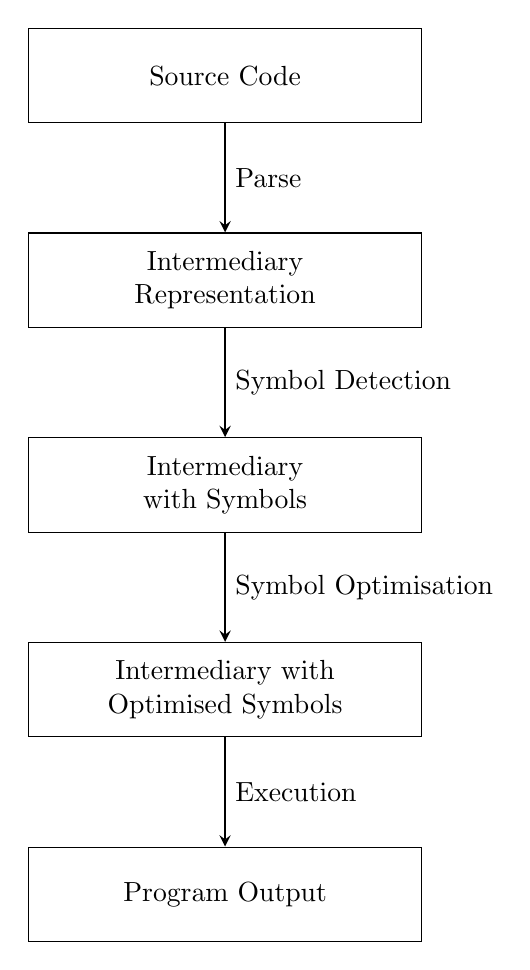
\begin{tikzpicture}[node distance=2.6cm]
        \node (source) [plain_box] {Source Code};
        \node (intermediary) [plain_box, below of=source] {Intermediary Representation};
        \node (intermediary_1) [plain_box, below of=intermediary] {Intermediary with Symbols};
        \node (intermediary_2) [plain_box, below of=intermediary_1] {Intermediary with Optimised Symbols};
        \node (execution) [plain_box, below of=intermediary_2] {Program Output};

        \draw [arrow] (source) -- node[anchor=west] {Parse} (intermediary);
        \draw [arrow] (intermediary) -- node[anchor=west] {Symbol Detection} (intermediary_1);
        \draw [arrow] (intermediary_1) -- node[anchor=west] {Symbol Optimisation} (intermediary_2);
        \draw [arrow] (intermediary_2) -- node[anchor=west] {Execution} (execution);
    \end{tikzpicture}
    \caption{How a Kihi program is executed.}
    \label{fig:kihi_execution_process}
\end{figure}
The implementation described in this project, which is also referred to as the Kihi Runner, is capable of directly handling Kihi source code. The execution process is outlined in figure \ref{fig:kihi_execution_process}, and as the figure shows, the source code is first parsed and transformed into an intermediary representation before execution. The details of the intermediary representation are discussed in section \ref{sec:implementation_intermediary_representation}. This intermediary is then optionally optimised through the process of symbol detection, and symbol optimisation which are the subjects of section \ref{sec:implementation_optimisation}. The details of the execution stage are omitted from the above figure due to desire for simplicity, but the process essentially involves selecting an executor, which can be understood as a virtual machine, and utilising it to execute the intermediary representation. The implementation supports three types of executors: a term rewriting based executor, a stack based executor, and a depreciated term rewriting based executor kept for posterity. The implementation details of the executor process and the executors are provided in section \ref{sec:implementation_executors}

\todo[inline]{
    maybe in background elaborate on what a virtual machine is?
}

\section{Configuration}
The Kihi Runner provides various configuration options available at compile time and run time. Compile time options are available through feature flags and run time options can be specified using command line flags. Feature flags make it possible to include or exclude various features such as the certain executors, CPU profiling, and output printing from the binary. This reduces the size of the binary and also removes unneeded features which might impact performance. This is especially true of output printing since formatting outputs incurs an noticeable runtime overhead. CPU profiling also incurs an, albeit minor, runtime overhead. The run time arguments are use to specify which executor to utilise, the degree of optimisation, and the number of outputs to print. More specific details of these configuration options are available in the project's readme.

\todo[inline]{
    move this:
    This intermediary representation is mostly identical to the grammar shown in figure \ref{fig:kihi_grammar} barring implementation details, debugging symbols, and optimisation mechanisms. The optimisation mechanisms are of particular interest and are discussed in greater detail in section \ref{sec:implementation_optimisation}.
    The executable takes as an argument the path to a text file contain Kihi source code, encoded in either UTF-8 or ASCII, and subsequently runs the program, emitting any outputs to standard output.
}

\section{Implementation Language}
This project was implemented in Rust. This decision was largely motivated by performance concerns and ease of use. Rust is considered a systems language and is designed with performance as a principal goal. An manifestation of this is manual control over memory in conjunction with a type system capable of guaranteeing memory safety. This provides the performance benefits of a low level language while retaining the safety benefits of a garbage collection. Furthermore, Rust also provides many features commonly found in functional programming languages, such as pattern matching, which significantly improve the ergonomics of the language especially in the context of programming language implementation as shown by the ubiquitous of such features throughout the codebase. Overall, these factors give Rust well earned respect as a language suitable for performance sensitive projects, and an especially compelling choice for this project.

\todo[inline]{Reference rust webpage?}

\section{Intermediary Representation}\label{sec:implementation_intermediary_representation}
The intermediary representation is essential identical to an abstract syntax tree of the grammar shown in figure \ref{fig:kihi_grammar} barring implementation details, debugging symbols, and optimisation mechanisms. The purpose of the intermediary representation is two fold. Firstly, it decouples the source code from the executable representation allowing room for the aforementioned differences. Secondly, it provides a common representation that can be interpreted by the various executors. An example of an intermediary representation is shown in figure \ref{fig:kihi_intermediary_representation_example_1}. The optimisation mechanisms introduced to the intermediary representation are the most interesting and are the subject of section \ref{sec:implementation_optimisation}. However, from the perspective of the intermediary representation they merely manifest as an additional term in the grammar denoted as `Symbol'.

\tikzstyle{arrow} = [thick,->,>=stealth]

\tikzstyle{program} = [rectangle, minimum width=2.8cm, minimum height=1cm, text centered, node contents=Program, draw=black]

\tikzstyle{abstraction} = [rectangle, minimum width=2.8cm, minimum height=1cm, text centered, node contents=Abstraction, draw=black]

\tikzstyle{apply} = [rectangle, minimum width=2.8cm, minimum height=1cm, text centered, node contents=Apply, draw=black]

\tikzstyle{left} = [rectangle, minimum width=2.8cm, minimum height=1cm, text centered, node contents=Left, draw=black]

\tikzstyle{right} = [rectangle, minimum width=2.8cm, minimum height=1cm, text centered, node contents=Right, draw=black]

\tikzstyle{copy} = [rectangle, minimum width=2.8cm, minimum height=1cm, text centered, node contents=Copy, draw=black]

\tikzstyle{drop} = [rectangle, minimum width=2.8cm, minimum height=1cm, text centered, node contents=Drop, draw=black]

\begin{figure}[htb]
    \centering
    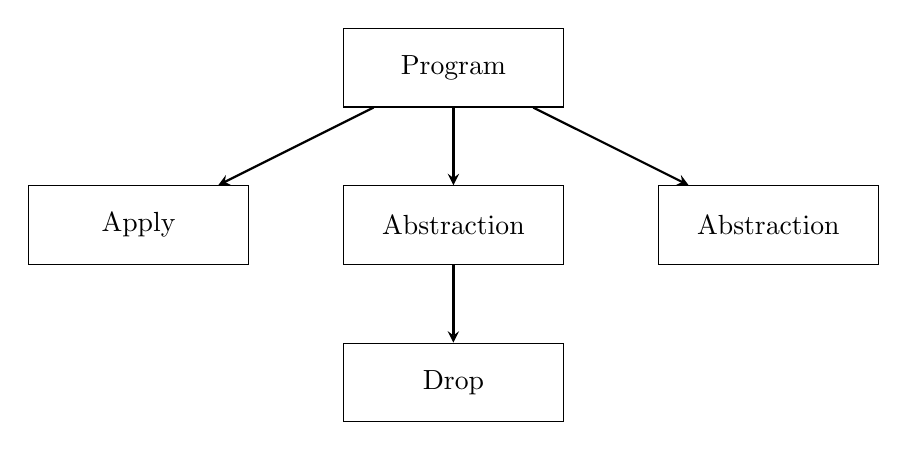
\begin{tikzpicture}[node distance=2cm]
        \node (program) [program];
        \node (2) [abstraction, below of=program];
        \node (1) [apply, left of=2, xshift=-2cm];
        \node (3) [abstraction, right of=2, xshift=2cm];
        \node (4) [drop, below of=2];

        \draw [arrow] (program) -- (1);
        \draw [arrow] (program) -- (2);
        \draw [arrow] (program) -- (3);
        \draw [arrow] (2) -- (4);
    \end{tikzpicture}
    \caption{Kihi intermediary representation of the program: \lstinline{apply (drop) ()}}
    \label{fig:kihi_intermediary_representation_example_1}
\end{figure}


% · → × → (· · ← (→ → (·) ×)) (· ← (· · ← ← ()) × → (· · ← (·) · ← ← () · ← (×)) · ← ← ()) (↓)


\section{Executors}\label{sec:implementation_executors}
Executors are used to compare the performance of various execution methods. They represent virtual machines that are capable of executing the intermediary representation and are essentially the implementations of the operational semantics shown in section \ref{sec:background_evaluation_methods}. In fact, an almost direct translation of the semantics presented in that section lies at the heart of this project's implementation. Furthermore, the algorithm used in this implementation is accurately represented by the pseudocode in figures \ref{fig:term_rewriting_pseudocode} and \ref{fig:stack_pseudocode}.

\subsection{Reduce Executor}
\begin{figure}[htb]
    \centering
    \begin{lstlisting}
execute_program(input: String):
    terms: []Term := parse_program(input)
    
    reductible_term: Index := find_reductible_term(terms)
    while (reductible_term != -1) {
        reduce_term(terms, reductible_term)
    }

find_reductible_term(terms: []Term):
    for i: Index in 0..|terms| {
        if terms[i] is 'apply'
            and terms[i+1] is abstraction => return i
        else if terms[i] is 'left'
            and terms[i+1] and terms[i+2] are abstractions => return i
        else if terms[i] is 'drop'
            and terms[i+1] => return i
        ... and so on for each inference rule
        }
    }
    return -1

reduce_term(terms: []Term, term: Index):
    if terms[index] is 'apply'
        terms[index..index+1] = terms[index+1]
    else if terms[index] is 'left'
        terms[index..index+2] = [terms[index+2], ...terms[index+1]]
    else if terms[index] is 'drop'
        terms[index..index+1] = []
    ... and so on for each inference rule
    \end{lstlisting}
    \caption{Pseudocode for a term rewriting based Kihi implementation}
    \label{fig:term_rewriting_pseudocode}
\end{figure}

The heart of the reduce executor algorithm is relatively simple. The reduce executor algorithm consists of only two steps. The first step is finding a reducible term, this means finding an operator directly followed by a sufficient number of abstractions. This corresponds to the \lstinline{find_reductible_term} function shown in figure \ref{fig:term_rewriting_pseudocode}. Secondly, if an reducible term is found the corresponding reduction rule is applied, otherwise if no such terms can be found the program halts. This process is repeated until the program halts.

\subsection{Stack Executor}
\begin{figure}[htb]
    \centering
    \begin{lstlisting}
execute_program(input: String):
    program: []Term := parse_program(input)
    
    stack: []Term := []
    
    while(|terms| != 0) {
        term := terms.pop()
        if term is abstraction => stack.push(term)
        else if term is 'apply' => program.append( stack.pop() )
        else if term is 'left' => {
            arg1 = stack.pop()
            arg2 = stack.pop()
            stack.push( [arg2] ++ arg2 )
        }
        ... and so on for each inference rule
    }
    \end{lstlisting}
    \caption{Pseudocode for a stack based Kihi execution}
    \label{fig:stack_pseudocode}
\end{figure}

The stack executor algorithm is equally simple or potentially even simpler. The algorithm consists of only a single step where the right most term in the program is inspected and the stack modified accordingly. For instance, when an abstraction is encountered it is pushed onto the stack, and when an apply is encountered an abstraction is popped off the stack and the abstraction's inner program appended to the terms. This is repeated until the right most term requires more arguments than there are values on the stack or the terms are exhausted.

Comparing the performance of executors is worthwhile because the implementations of the term rewriting semantics and the stack semantics, which hereinafter are referred to as the reduce executor and stack executor, are substantially different from a mechanical perspective. The reduce executor algorithm can be decomposed into two parts: reducible term finding and term reduction. In contrast, the stack executor algorithm simply consists of reduction.  Hypothetically it would appear that the stack executor would perform significantly better than the reduce executor simply due to the additional $\Theta(n)$ reducible term finding operation required before each reduction, as shown by line 4 of figure \ref{fig:term_rewriting_pseudocode}. Whether this holds in practice is the topic of chapter \ref{C:evaluation}.

As mentioned in earlier sections, a third executor also exists. This third executor is a previous implementation of the term rewriting operational semantics and is primarily kept for posterity. However, it also provides an useful indicator of how much the performance can vary when the underlying operational semantics remain the same.


\section{Optimisation}\label{sec:implementation_optimisation}
\tikzstyle{symbol} = [rectangle, minimum width=2.8cm, minimum height=1cm, text centered, draw=black]

\begin{figure}[htb]
    \centering
    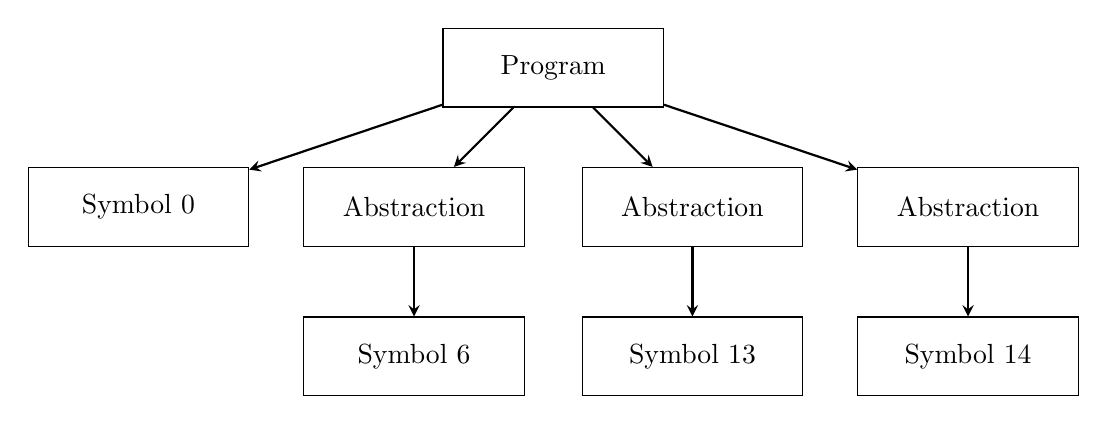
\begin{tikzpicture}[node distance=2.5cm]
        \node (program) [program];
        \node (2) [abstraction, below left of=program];
        \node (3) [abstraction, below right of=program];
        \node (1) [symbol, left of=2, xshift=-1cm] {Symbol 0};
        \node (4) [abstraction, right of=3, xshift=1cm];

        \node (2c) [symbol, below of=2, yshift=0.6cm] {Symbol 6};
        \node (3c) [symbol, below of=3, yshift=0.6cm] {Symbol 13};
        \node (4c) [symbol, below of=4, yshift=0.6cm] {Symbol 14};

        \draw [arrow] (program) -- (1);
        \draw [arrow] (program) -- (2);
        \draw [arrow] (program) -- (3);
        \draw [arrow] (program) -- (4);

        \draw [arrow] (2) -- (2c);
        \draw [arrow] (3) -- (3c);
        \draw [arrow] (4) -- (4c);
    \end{tikzpicture}
\vspace*{1cm}

\begin{tikzpicture}[cell/.style={rectangle,draw=black},
space/.style={
        minimum height=1.5em,matrix of nodes,row sep=-\pgflinewidth,column sep=-\pgflinewidth,
        column 1/.style={font=\ttfamily}
    },
    text depth=0.5ex,text height=2ex,nodes in empty cells]

\matrix (first) [space, 
    column 1/.style={nodes={cell, minimum width=1.5cm}},
    column 2/.style={nodes={cell, minimum width=12cm}}
] {
Symbol   & Terms \\
0   & apply right copy right \\
1   & apply apply left \\  
2   & right right \\  
3   & apply \\  
4   & copy \\  
5   & symbol\_2 (symbol\_3) symbol\_4 \\  
6   & symbol\_1 (symbol\_5) \\  
7   & apply left \\  
8   & apply apply left left \\  
9   & symbol\_8 () \\  
10   & copy right  \\  
11   & apply left left \\  
12   & symbol\_1 (symbol\_3) symbol\_11 () symbol\_7 (symbol\_4) \\   
13   & symbol\_7 (symbol\_9) symbol\_10 (symbol\_12) symbol\_11 () \\   
14   & drop \\  
};

\end{tikzpicture}
    \caption{Kihi Intermediary Representation}
    \label{fig:kihi_intermediary_representation}
\end{figure}

\tikzstyle{startstop} = [rectangle, rounded corners, minimum width=3cm, minimum height=1cm,text centered, draw=black, fill=red!30]
\tikzstyle{io} = [trapezium, trapezium left angle=70, trapezium right angle=110, minimum width=3cm, minimum height=1cm, text centered, draw=black, fill=blue!30]
\tikzstyle{process} = [rectangle, minimum width=3cm, minimum height=1cm, text centered, draw=black, fill=orange!30]
\tikzstyle{decision} = [diamond, minimum width=3cm, minimum height=1cm, text centered, draw=black, fill=green!30]
\tikzstyle{arrow} = [thick,->,>=stealth]

\begin{figure}[htb]
    \centering
    \begin{tikzpicture}[cell/.style={rectangle,draw=black},
    space/.style={
            minimum height=1.5em,matrix of nodes,row sep=-\pgflinewidth,column sep=-\pgflinewidth,
            column 1/.style={font=\ttfamily}
        },
        text depth=0.5ex,text height=2ex,nodes in empty cells]

    \matrix (first) [space, 
        column 1/.style={nodes={cell, minimum width=5cm}},
        column 2/.style={nodes={cell, minimum width=2.3cm}},
        column 3/.style={nodes={cell, minimum width=7cm}}
    ] {
    \textbf{Program}   & \textbf{Arguments} & \textbf{Optimised Representation}  \\
    left & 2 & ((arg\_1) arg\_0) \\
    right & 2 & (arg\_0 (arg\_1)) \\
    copy & 1 & (arg\_0) (arg\_0) \\
    drop & 1 & \\
    apply right copy right & 2 & arg\_0 (arg\_1) (arg\_0 (arg\_1)) \\
    apply apply left & 2 & apply (arg\_1) arg\_0 \\  
    right right & 3 & (arg\_0 (arg\_1) (arg\_2)) \\  
    };

    \end{tikzpicture}
    \caption{The optimised representations of some example programs}
    \label{fig:kihi_symbol_optimisation}
\end{figure}

The most significant contribution of this project is the creation of an approach for optimising Kihi programs. The approach essential involves replacing subprograms in Kihi with a potentially more efficient representation. This is accomplished in a two stage process. This is accomplished in two stage process. First, candidate subprograms are found through symbol detection and secondly these candidates are optimised using symbol optimisation. The subprograms are replaced by their corresponding symbols which can then executed using the representations created by the symbol optimisation process.

The symbol optimisation process essentially amounts to symbolic execution with placeholder inputs. The output of this execution provides an direct representation of the program's output parametric on the inputs. The symbolic execution is a limited form of stack execution where the `apply' operator can only be evaluated when the abstraction captures a statically known program. The output representation provides a template for the program's output given specific arguments. This allows for potentially faster execution since a simple find and replace procedure can be used to determine the output of executing a program given certain arguments rather than ordinary execution. Figure \ref{fig:kihi_symbol_optimisation} shows the output of this process for some small sample programs. 

\begin{figure}[htb]
    \centering
    \begin{lstlisting}
execute_program(input: String) -> Representation:
    program: []Term := parse_program(input)
    
    stack: []Term := []
    
    while(program is not empty and one of the cases below is true) {
        term := program.pop()
        if term is abstraction => {
            stack.push(term)
        }
        else if term is 'apply' and stack.peek() has known value => {
            arg1 = stack.pop()
            program.append( stack.pop() )
        }
        else if term is 'left' => {
            while(stack has insufficient arguments) {
                stack.push(placeholder_value)
            }
            arg1 = stack.pop()
            arg2 = stack.pop()
            stack.push( [arg2, ...arg1] )
        }
        ... and so on for each inference rule
    }

    return [...program, ...stack]
    \end{lstlisting}
    \caption{Pseudocode for a symbol optimisation}
    \label{fig:symbol_optimisation_pseudocode}
\end{figure}

The symbol detection process is designed to decompose the program into symbols that can be meaningfully optimised. There are many ways to decompose a program, however the algorithm utilised in the Kihi Runner is relatively simple. It simply combines any sequence of operators unbroken by abstractions into a single symbol. This is applied to the entire program and is recursively applied to the abstractions within programs. The output of this process when applied to the program in figure \ref{fig:kihi_example} is shown in figure \ref{fig:kihi_intermediary_representation_example_2}.

This overall strategy to optimisation is general and encourages further experimentation and research. The specific algorithms used for symbol detection and optimisation are not restricted to the ones utilised in this project. There are potentially more complex algorithms capable of handling more complex subprograms, this topic is discussed in further detail in chapter \ref{C:future_work}.

The origins of this approach are attempts at optimising the performance of the initial version of the Kihi Runner. In particular, they arose from initial attempts are optimising the Kihi Runner's performance on the count program presented in figure \ref{fig:kihi_example}. One such attempt was an symbol detection and symbol optimisation algorithm tailored to numbers. Although never completed, that algorithm would have been able to decode the church encoding of numbers and common operations such as addition. This would have allowed for a Kihi program to be efficient executed using basic assembly instructions, which are likely several magnitudes faster than ordinary execution. However, before this was fully developed it was generalised into the form that appears here.

\todo[inline]{Talk about why this might be faster than the ordinary execution}.

\todo[inline]{AST for the optimised representations}